
\chapter{Метод исследования}

В работе движение жидкости моделируется численными решениями полных уравнений Навье-Стокса. Все динамически существенные масштабы разрешаются явно, что освобождает от необходимости подбора замыкающих соотношений и эмпирических констант. Прямое численное моделирование зарекомендовало себя эффективным методом изучения пристенных турбулентных течений. Подробный численный анализ ряда пристенных течений показал, что численные решения уравнений Навье-Стокс с высокой точностью воспроизводят наблюдаемые в экспериментах особенности движения. Существенным достоинством численных методов при изучении турбулентных структур является то, что расчет дает полную информацию о течении. Изучаемые в работе переходные режимы течения наблюдаются при небольших значениях числа Рейнольдса (~2000) и доступны для численного анализа даже на персональном компьютере. 

Существенный вклад в развитие численных методов решения задач гидродинамической устойчивости и расчета гидродинамических течений внесли отечественный математики и механики \cite{Lad1970, Jud1984, Bab1986, Ger1972, Sch1973, Gold1977, Bel1984, Sch2010, Kul2014}. Расчеты трехмерных турбулентных течений наиболее активно проводились группой под руководством Б.Л. Рождественского в ИПМ им. Келдыша [(Rog1973), Rog1984, Rog1985, Pon1988, Pri1987, (Rog1987), Pri1991, (Pri1992)] и Н.В. Никитиным в НИИ механики МГУ []. На западе наиболее интенсивные расчеты течения в плоском канале выполнены в группе под руководством П. Моина в Стэнфордском университет [Moin1978, Moin1982, Kim1987]. 

Наиболее эффективные численные алгоритмы разработаны для моделирования движения жидкости в областях простой формы. Пристенные турбулентные течения наиболее полно исследованы в плоском канале -- между двумя параллельными плоскостями -- и в круглой трубе. В типичной постановке ищутся решения, удовлетворяющие условию периодичности вдоль потока, а в случае плоского канала и в трансверсальном направлении. Такая постановка хорошо себя зарекомендовала при расчете характеристик развитых турбулентных течений, устанавливающихся на большом удалении от входа в трубу или канал. Применение условий периодичности снимает вопрос постановки условий на открытых границах расчетной области, снимает необходимость расчета движения жидкости в переходной области течения и позволяет получить характеристики развитых турбулентных течений в расчетной области небольшого размера. Расчеты в пограничном слое и в круглой трубе с постановкой условий на входе и выходе из расчетной области (без условия периодичности вдоль потока) также проводились, но для выхода на установившийся режим течения они требуют значительно больше вычислительных ресурсов [Fazel1990a,b, Clocker1993, Никитин1994в, 1995].  

Общепринятым подходом при построении дискретной системы уравнений при расчете движения жидкости в трубах и каналах с условием периодичности является представление неизвестных в тригонометрическом базисе по однородным направлениям. Дискретизация системы уравнений выполняется методом Галеркина, обоснованным в работе Г.И. Петрова [Pet1940]. При этом основная сложность алгоритма оказывается связана с вычислением нелинейных слагаемых, что требует свертки рядов. Наиболее эффективные алгоритмы, позволяющие вычислить свертку рядов, основаны на применении быстрого преобразования Фурье [Kuli1965]. 

В работах [] для аппроксимации неивестных в нормальном к стенке направлении применялись полиномы Чебышева. 

В другом подходе уравнения движения приближаются конечными разностями. Конечно-разностные методы уступают спектральным при моделировании предтурбулентных режимов течения, для которых свойственны достаточно гладкие поля скорости и отсутствие мелкомасштабной составляющей движения [Orzag1971a]. Однако в развитых турбулентных течениях число гармоник Фурье и число точек в сетке, необходимые для того, чтобы достаточно точно приблизиться поле скорости, оказываются сравнимы, и конечно-разностные методы не уступают спектральным в эффективности [Ray1991]. К преимуществам конечно-разностных методов можно отнести то, что они достаточно просты в реализации, сравнительно легко адаптируются к изменению геометрии расчетной области и граничных условий. Метод построения конечно-разностной дискретизации уравнений Навье-Стокса в ортогональной системе координат предложен в работе [Никитин2006]. Предложенный метод сохраняет ряд консервативных свойств исходной системы уравнений. В частности, нелинейные слагаемые не производят кинетической энергии, что особенно важно при расчете турбулентных течений. В настоящей работе расчеты выполнены методом [Nik2006]. 


\section{Математическая постановка задачи} \label{math_section}

Рассматривается течение вязкой несжимаемой жидкости в прямой трубе круглого сечения. Движение описывается уравнениями Навье-Стокса и неразрывности:
\begin{equation} \label{NS_eq}
\pd{\v}{t} = - (\v \nabla) \v - \frac{1}{\rho}\grad p + \nu \nabla^2 \v,
\end{equation}
\begin{equation} \label{div_eq}
\nabla \cdot \v = 0.
\end{equation}
Здесь $\v$ --- поле скорости, $p$ --- давление, $\rho$ --- плотность жидкости, $\nu$ --- кинематический коэффициент вязкости, $t$ --- время. 

Задача решается в цилиндрической системе координат $(x,r,\theta)$. На стенках трубы, имеющей радиус $R$, ставится условие прилипания:
\begin{equation} \label{bc1_eq}
\v \big|_{r=R} = 0.
\end{equation}

В продольном направлении на поле скорости налагается условие периодичности с периодом $L_x$:
\begin{equation} \label{bc2_eq}
\v \big|_{x+L_x} = \v \big|_{x}
\end{equation}
Из \eqref{NS_eq} следует, что давления в этом случае представляется в виде
\begin{equation} \label{bc3_eq}
p = - D_p(t)x + q, \ \ \ \  q\big|_{x+L_x} = q\big|_{x},
\end{equation}
где $D_p$ --- внешний градиент давления, вызывающий движение жидкости. 

Значение $D_p$ определяется из условия постоянства средней скорости течения $U_m$: 
\begin{equation} \label{Q_eq}
\frac{\partial U_m}{\partial t} = 0.
\end{equation}
Значение $U_m$, в свою очередь, определяется начальными условиями:
\begin{equation} \label{ic_eq}
\v \big| _{t = 0} = \v_0. 
\end{equation}

Безразмерным параметром системы является число Рейнольдса, введенное следующим образом:
\begin{equation} \label{Re_eq}
\Re = \frac{2 R U_m}{\nu}. 
\end{equation}

Задача поставлена традиционным образом для прямого расчета развитых турбулентных течений в трубах и каналах. В такой постановке удается воспроизводить характеристики течения, устанавливающегося на большом удалении от входа в трубу, решая уравнения движения в ограниченной расчетной области. Условие периодичности вдоль трубы освобождает от необходимости устанавливать условия на входе и выходе из трубы. В тоже время, увеличивая длину периода $L_x$, можно минимизировать влияние этого условия на поток. Для того, чтобы иметь возможность воспроизвести в расчете локализованные турбулентные структуры, необходимо выбирать протяженность расчетной области $L_x$ достаточно большой, не менее $40$ диаметров трубы. 


\section{Численный метод} \label{num_method}

Поставленная задача решается численно конечно-разностным методом \cite{Nikitin2006}. Метод формулируется относительно уравнений движения \eqref{NSeq_Re}, преобразованного к виду:
\begin{equation}\label{NSeq_om}
\pd{\v}{t} =  \v \times \om  - \i b - \grad \Pi - \frac{1}{\Re} \rot \om.
\end{equation}
Здесь $\om = \rot \v$ --- вектор завихренности, посчитанный по полю скорости $\v$; $\Pi = p + \v^2/2$ --- полное кинематическое давление. Эквивалентность уравнений \eqref{NSeq_Re} и \eqref{NSeq_om} следует из векторных тождеств:
\begin{equation*}
-(\v, \nabla) \v = \v \times \rot \v - \grad \frac{\v^2}{2},
\end{equation*}
\begin{equation*}
\Laplace \v = \grad \div \v - \rot \rot \v.
\end{equation*}

Задача решается в цилиндрической системе координат $(x,r,\theta)$. Расчетная область в пространстве $(x,r,\theta)$ имеет форму параллелепипеда:
\begin{equation}
0 < x < L_x, 0 < r < 1, 0 < \theta < 2\pi.
\end{equation}
При решении уравнений в этих переменных необходимо дополнительно установить условие периодичности в направлении $\theta$ и условие ограниченности решения при $r=0$.

В пространстве $(x,r,\theta)$ в расчетной области вводится прямоугольная расчетная сетка, однородная в направлениях $x$ и $\theta$. В радиальном направлении вводится растяжение сетки, что позволяет уменьшить её шаг вблизи стенки. Во всех расчетах, представленных в работе, параметр растяжения выбран таким образом, что размер ячейки в радиальном направлении около стенки в 4 раза меньше, чем в центре трубы. 

При дискретизации уравнений применен подход, при котором различные неизвестные определяются в различных точках сетки. Так, давление $p$ относится к центру ячеек. Компоненты вектора скорости $v_k$ относятся к центрам граней, нормальных к направлению $k$. Компоненты вектора завихренности $\omega_k$ относятся к центрам ребер, параллельных направлению $k$. При таком подходе говорят, что неизвестные определены на смещенных или разнесенных сетках. Он позволяет естественным образом ввести аппроксимацию уравнений второго порядка точности по пространственным переменным.

Пространственная дискретизация вводится таким образом, что сохраняется ряд важных консервативных свойств исходной системы. В частности, тождественно равна нулю дивергенция вязких слагаемых в \eqref{NSeq_Re}, что гарантирует, что это слагаемое не производит массы. Также тождественно равна нулю завихренность градиента давления, что обеспечивает отсутствие влияния давления на эволюцию завихренности непосредственно. 

При моделировании турбулентных течений важно аккуратно воспроизводить изменение кинетической энергии системы. Описывающее его уравнение возникает в результате скалярного умножения на $\v$ уравнений движения \eqref{NSeq_Re} с последующим суммированием по всей расчетной области. Важным свойством системы является то, что в уравнении Навье-Стокса для несжимаемой жидкости градиент периодической составляющей давления и нелинейные слагаемые не производят кинетической энергии, а лишь перераспределяют уже существующую. В конечно-разностной постановке строго выполняются тождества, выражающие этот факт, справедливые при \eqref{eq0_Re}, \eqref{bc0_Re}, \eqref{bc1_Re}:
$$
\int_V \v \cdot \grad p\ d\tau= \int_V \grad (\v p) d\tau = \int_{\Sigma} p v_n d\sigma = 0, 
$$
$$
\int_V \v \cdot (\v, \nabla) \v\ d\tau = \int_V (\v, \nabla)\frac{\v^2}{2}\ d\tau = \int_V \grad (\v \frac{\v^2}{2}) d\tau = \int_{\Sigma} \frac{\v^2}{2} v_n d\sigma = 0.
$$
Здесь $V$ --- расчетная область, $\Sigma$ --- её граница, $v_n$ --- нормальная составляющая скорости на границе. Также строго выполняется дискретный аналог уравнения изменения полной кинетической энергии $E$, записанного в следующем виде:
\begin{equation} \label{Eeq}
\frac{d E}{d t} = - \frac{1}{2}bV - \frac{1}{\Re} \int_{V} \omega^2 d\tau,
\end{equation}
$$
E = \frac{1}{2}\int_{V} \v^2 d\tau.
$$
Изменение полной энергии происходит за счет внешнего градиента давления $b$ и вязкой диссипации. 

Интегрирование по времени выполняется полу-неявным методом Рунге-Кутты третьего порядка точности \cite{Nikitin2006third}. В силу нелинейности оператора Навье-Стокса реализовать полностью неявный метод продвижения по времени затруднительно. Однако наибольшая жесткость системы на достаточно подробных сетках связана с вязким слагаемым. В силу их линейности они могут быть разрешены неявно в то время, как другие слагаемые в операторе Навье-Стокса разрешаются явно. Такой подход называется полу-неявным и позволяет существенно увеличить допустимый временной шаг в сравнении с явными методами. Реализованный алгоритм допускает автоматический выбор шага интегрирования исходя из условия сохранения локальной точности получаемого решения. Таким образом, шаг интегрирования автоматически адаптируется к изменениям в структуре течения, и не требует явного его задания во время счета. 

Неточность выполнения закона сохранения энергии в конечно-разностной постановке может быть следствием не только несовершенства пространственной дискретизации, но и результатом неточности выполнения интегрирования по времени. В типовых расчетах движения идеальной жидкости метод Рунге-Кутты третьего порядка обладает диссипативным свойством --- неточности выполнения шага по времени ведут лишь к потере кинетической энергии, но не её производству \cite{Nikitin2006}. Можно ожидать, что это свойство в некоторой степени сохраняется при решении уравнений Навье-Стокса используемым в работе методом. 

На каждом шаге по времени возникает необходимость по известному полю скорости $\v$ определить полное давление $\Pi$. Для этого необходимо решить уравнение Пуассона, возникающее при условии несжимаемости \eqref{eq0_Re} в результате применения оператора дивергенции к уравнениям движения \eqref{NSeq_om}. Уравнение для определения давления имеет вид:
\begin{equation}\label{P_eq}
\Laplace \Pi = \div \tilde \v,
\end{equation}
$$
\tilde \v =  \v \times \om - \frac{1}{\Re} \rot \om.
$$
Правая часть уравнения \eqref{P_eq} определяется по полю скорости $\v$. Давление также удовлетворяет условию периодичности в направлениях $x$ и $\theta$. На оси трубы значение давления ограничено. Условие на твердой стенке возникает в результате проектирования уравнения \eqref{NSeq_om} на направление нормали $n$:
$$
\pd{p}{n} = \tilde v_n.
$$


Простая геометрия расчетной области позволяет применять прямые методы решения возникающей в результате дискретизации уравнения \eqref{P_eq} линейной системы. Метод решения задачи для давления основан на применении быстрого преобразования Фурье в направлениях $x$ и $\theta$, в которых решение меняется периодическим образом и сетка имеет постоянный шаг. В радиальном направлении система решается методом прогонки. Общая сложность решения задачи для давления составляет $O(N \log N)$, где $N$ --- количество ячеек в расчетной сетке. Решение задачи для давления составляет основную вычислительную сложность используемого метода. 


\section{Реализация численного метода}

Пакет программ, реализующий описанный в предыдущем разделе численный метод, написан на языке программирования fortran77 Н.В.\,Никитиным. Численный метод используется в лаборатории общей аэродинамики института механики МГУ уже более 20 лет и хорошо себя зарекомендовал. Программный код отлажен в процессе решения большого числа задач. В частности, с его помощью получены результаты, приведенные в работе \cite{Nikitin2006}, демонстрирующие согласие характеристик турбулентных потоков, полученных в расчетах и экспериментальным путем. Адекватность численного метода и качество его программной реализации подтверждают также результаты расчетов течения жидкости в трубе при переходных $\Re$, представленные в следующем разделе. В соответствии с результатами эксперимента, турбулентность принимает форму локализованных структур, характеристики которых совпадают с характеристиками турбулентного порыва.

Помимо последовательного варианта программы реализован параллельный, позволяющий выполнять расчеты на кластерных вычислительных системах с распределенной памятью. Для коммуникации между процессами, запущенными на различных узлах вычислительной системы, использован интерфейс передачи сообщений MPI (<<Message Passing Interface>>). Параллельная программа реализована следующим образом. Труба в продольном направлении делится на равные участки, каждый из которых хранится в памяти и обрабатывается собственным вычислительным процессом. На каждом шаге по времени каждый процесс обменивается граничными условиями с двумя соседями, что требует $O(1)$ пересылок. При решении задачи для давления необходимо перераспределить данные между процессами, при этом каждый процесс обменивается сообщением с каждым, что требует $O(M)$ пересылок, $M$ --- число процессов. С организацией обмена сообщениями между процессами связаны существенные затраты при выполнении программ на вычислительных кластерах. В  реализованном алгоритме при выполнении одного шага по времени каждый процесс совершает $O(M)$ пересылок.

Значительная часть расчетов была выполнена на суперкомпьютерах <<Чебышев>> и <<Ломоносов>> суперкомпьютерного комплекса МГУ. Характерное число вычислительных ядер, задействованных в расчетах, от 32 до 64, что позволяет увеличить скорость расчетов примерно в 10 раз. В зависимости от архитектуры вычислительной системы, на один вычислительный узел приходится от 4 до 8 вычислительных ядер.

Значительная часть кода, необходимого при анализе полученных результатов и управлении численными экспериментами, в том числе реализующая метод поиска решения на сепаратрисе (см. раздел \ref{edge_seq}) и метод поиска условно периодических траекторий (см. раздел. \ref{Newton_seq}), была написана на высокоуровневом языке python автором диссертации. Применение указанных методов сводится к последовательному обращению к программе расчета движения жидкости с правильно подобранными начальными данными. 


\section{Методические расчеты} \label{puff_calc}

\begin{figure}[h]
\center{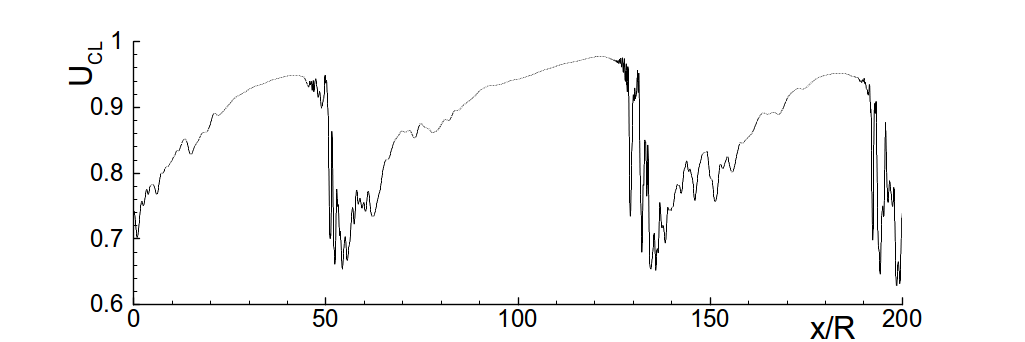
\includegraphics[width=0.9\linewidth]{exper2.png}}
\center{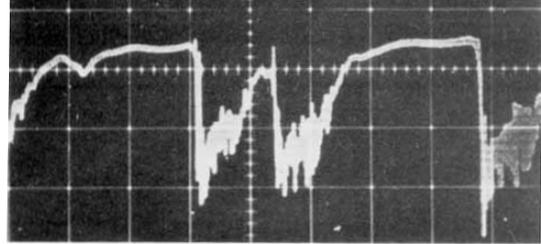
\includegraphics[width=0.68\linewidth]{exper3.png}}
\caption{Сравнение результатов численного расчета и эксперимента. Изображена скорость на оси трубы. Верхний график построен по результатам численного моделирования, выполнено Н.В. Никитиным применяемым в работе методом. Нижний график получен в эксперименте \cite{Wygnanski1973}.}
\label{exper_img}
\end{figure}

В разделе приведены результаты расчетов движения жидкости в круглой трубе в диапазоне $1670\leqslant Re\leqslant 2800$, полученные при $L_x=200$ с пространственным разрешением $2048 \times 64 \times 128$ ячеек в продольном, радиальном и угловом направлении соответственно. Расчеты на более грубой сетке $1024\times32\times64$ во всех рассмотренных случаях дают результаты совпадающие качественно и близкие количественно.

\begin{figure}[h]
\center{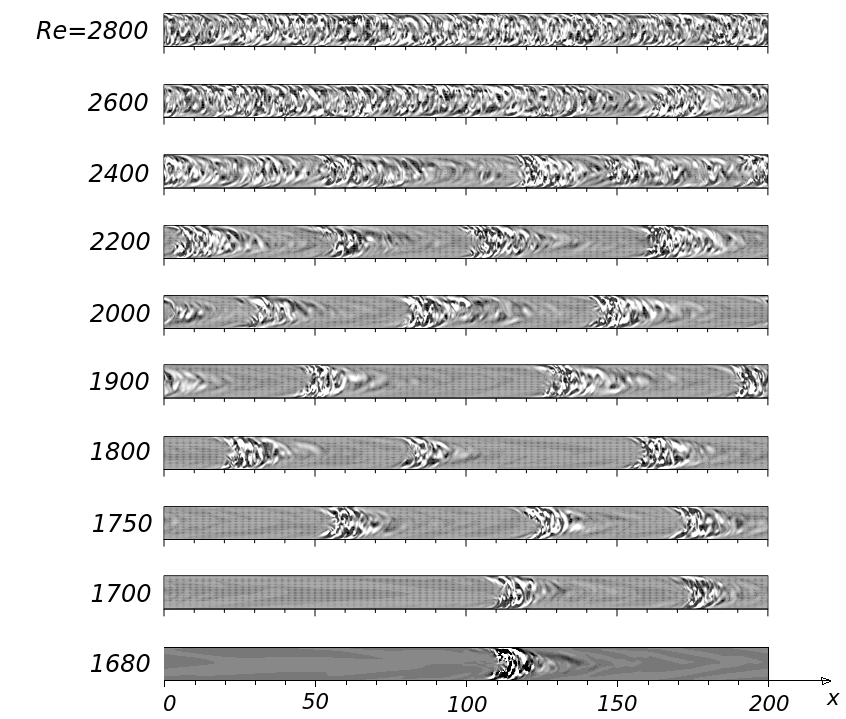
\includegraphics[width=1\linewidth]{puffs.png}}
\caption{Перемежаемый характер турбулентности в трубе в диапазоне переходных чисел Рейнольдса.}
\label{puffs_img}
\end{figure}

Стартуя с начальных данных в виде некоторого трехмерного возмущения течения Пуазейля, уравнения Навье--Стокса интегрируются до выхода решения на тот или иной режим. Установление решения, отвечающего турбулентному течению, происходит в том случае, когда амплитуда начального возмущения достаточно велика, в противном случае возмущения затухают со временем, и решение в конечном итоге возвращается к ламинарному течению Пуазейля. Турбулентный режим за пределами диапазона переходных чисел Рейнольдса $Re\geqslant3000$ имеет вид статистически стационарного процесса и не зависит от конкретного вида начальных условий, при которых он был получен. Течение при этом однородно в продольном направлении, его статистические характеристики согласуются с имеющимися экспериментальными данными. При $\Re\leqslant2600$ в распределении скорости вдоль трубы появляется неоднородность, которая при $\Re\lesssim2200$ приобретает форму двигающейся вдоль трубы цепочки из нескольких пространственно-локализованных структур, разделенных участками ламинарного течения. Конкретное число получающихся в решении турбулентных структур зависит от начальных условий. Кроме того, как было отмечено выше, это число может меняться в процессе эволюции в результате исчезновения или деления отдельных структур. Получаемые в расчетах пространственно-локализованные турбулентные структуры хорошо согласуются с наблюдаемыми в экспериментах турбулентными порывами, что позволяет нам пользоваться этим их наименованием (см. рис. \ref{exper_img}). Отметим, что турбулентные порывы формируются и на некотором отрезке времени существуют в расчетах и при $Re<2000$, вплоть до $Re=1670$. Однако, в этом случае не только число порывов в пределах расчетной области, но и время их существования является случайной величиной и зависит от конкретных начальных условий. Представленная на фиг.~\ref{puffs_img} визуализация рассчитанных течений в диапазоне $1680\leqslant Re\leqslant2800$ демонстрирует эволюцию локализованных структур при изменении числа Рейнольдса.

